\documentclass[11pt,a4paper]{article}
\usepackage{booktabs}
\usepackage{longtable}
\usepackage{array}
\usepackage{amsmath}
\usepackage{graphicx}
% Manual page layout (geometry.sty is not installed in this MiKTeX tree)
\setlength{\textwidth}{16.8cm}
\setlength{\textheight}{23.8cm}
\setlength{\oddsidemargin}{-0.44cm}
\setlength{\evensidemargin}{-0.44cm}
\setlength{\topmargin}{-0.7cm}
\setlength{\headheight}{0pt}
\setlength{\headsep}{0.3cm}
\setlength{\footskip}{0.8cm}
\setlength{\belowcaptionskip}{7pt}
\setlength{\itemsep}{2pt}
\setlength{\topsep}{2pt}
\setlength{\leftmargini}{1.5em}
\newcommand{\pp}{percentage points}
\pagestyle{plain}

\begin{document}

\begin{center}
{\Large\bfseries COMP4163 Course Project --- Final Report}\\[4pt]
{\large Degradation in plain networks and what residual connections fix}\\[8pt]
\begin{tabular}{@{}rl@{}}
Team: & group 11 \\
Members: & Chen Letian 2330026013 \\
         & Zhang Yiyang 2430024331 \\
         & Liu Chuanliang 2330013021 \\
         & Liu Yilin 2430026139 \\
\end{tabular}\\[8pt]
Date: 18 December 2026
\end{center}

\vspace{-2pt}
\noindent\rule{\textwidth}{0.4pt}

\section{Introduction}

Adding layers to a neural network is supposed to make it more expressive, and
more expressive should mean lower error. In 2016 He, Zhang, Ren and Sun
reported a case where it does not: on CIFAR-10, a plain convolutional network
with 56 layers has a \emph{higher training error} than an otherwise identical
20-layer network trained with the same recipe. The deeper network does not
merely generalise worse --- it does not even fit the data it is trained on. The
authors call this the degradation problem, and their fix, residual learning, is
one of the most consequential architectural ideas in modern computer vision.

The argument has two parts and it is worth separating them, because the second
is what makes the paper more than a negative result.

First, degradation is not overfitting. A deep network that memorised its
training set would show \emph{low} training error and \emph{high} test error.
The phenomenon reported instead is that both errors rise with depth, which
locates the problem in optimisation rather than in generalisation. This is why
the paper rules out the obvious explanations: the deeper network can represent
anything the shallower one can (an identity stack is available), and the
gradients do not vanish, so neither capacity nor gradient flow explains it.

Second, the fix. A residual block computes $y = F(x) + x$ rather than
$y = F(x)$, so the block only has to learn a residual. If the best thing for a
group of layers to do is nothing, the residual can be driven to zero, and the
optimiser no longer has to discover an identity mapping through a stack of
non-linear layers. The paper's headline numbers are on ImageNet, but the
cleanest evidence for the mechanism is on CIFAR-10, and that is what we
reproduce.

The audience for this report knows the course material but not this paper, so
we give the recipe and our implementation in enough detail to be checked, then
the reproduction, then a controlled experiment that asks whether the
degradation survives when each depth is allowed its own learning rate.

\section{What we reproduce, and how strong the paper's evidence is}

We reproduce the CIFAR-10 evidence: Figure~6 (left and middle) and the
ResNet-20 and ResNet-56 rows of Table~6. Concretely, we train four networks ---
plain-20, plain-56, ResNet-20 and ResNet-56 --- with three seeds each, twelve
runs in total, and compare (i) the training and test curves against Figure~6
and (ii) the test errors at iteration 64{,}000 against Table~6.

An honest reproduction has to say how much evidence stands behind the number it
is compared with, and here the paper is thinner than its presentation suggests.
Figure~6 shows one curve per depth and the paper does not state how many runs
are behind it. The Table~6 entries for the depths we reproduce are single runs.
Only ResNet-110 is trained five times, and there the paper reports both the best
value (6.43\%) and the mean with a standard deviation (6.61$\pm$0.16). No seed
spread is reported for any of the four networks we train. Our three seeds per
network are therefore not redundant with the paper: they add a spread that the
original evidence does not contain, and that spread is what decides whether a
difference between two networks is real.

\section{The recipe, and the choices the paper leaves open}

The CIFAR-10 recipe of Sec.~4.2 is: SGD with momentum 0.9 and weight decay
$10^{-4}$; batch size 128; He (MSRA) initialisation; batch normalisation after
every convolution; no dropout; the learning rate starts at 0.1 and is divided
by ten at iterations 32{,}000 and 48{,}000; training stops at 64{,}000
iterations, a point the paper says ``is determined on a 45k/5k train/val
split''. Data augmentation is a 4-pixel zero pad followed by a random
$32\times32$ crop and a random horizontal flip; at test time a single view of
the un-augmented image is used, with a per-pixel mean subtracted. The 110-layer
network alone gets a short warm-up, which does not concern us.

Several choices are left open, and our decisions are:

\begin{center}
\begin{tabular}{@{}p{3.6cm}p{5.2cm}p{6.4cm}@{}}
\toprule
\textbf{Open choice} & \textbf{What the paper says} & \textbf{Our decision} \\
\midrule
Which 5{,}000 images form the validation split & Not specified & Concatenate the five training batches in the order they are stored and hold out the last 5{,}000 \\
Whether the networks saw 45{,}000 or 50{,}000 images & Places the 64k stopping point on a 45k/5k split but does not say what the networks were trained on & Train on the first 45{,}000; the topic card notes they were ``likely trained on all 50{,}000'' \\
Number of runs per network & Not stated & Three per network, three for the tuned extension \\
How the Figure~6 training error is measured & Not stated & Report both an evaluation-mode error on the 45{,}000 images and a running error on the augmented training minibatches \\
Interface between the epoch and the schedule & Epochs are not used & Everything counted in iterations; an epoch is 351 iterations, i.e.\ $45{,}000/128$ with the last partial batch dropped \\
\bottomrule
\end{tabular}
\end{center}

\section{Our pipeline}

The networks are the ones of the paper's CIFAR-10 section: $6n+2$ weighted
layers, with one $3\times3$ convolutional stem producing 16 channels, then three
stages of $2n$ $3\times3$ convolutions on $32\times32$, $16\times16$ and
$8\times8$ feature maps with 16, 32 and 64 channels, a global average pool and a
single fully connected layer. This gives 269{,}722 parameters at depth 20 and
853{,}018 at depth 56, and the two counts are identical for the plain and the
residual networks, which is the point of using identity shortcuts with
zero-padding where the number of channels increases (the paper's option A).

Training follows the protocol of the topic card. One epoch is 351 iterations
and the schedule is counted in iterations, so 64{,}000 iterations is 183
epochs, the last one partial. After every epoch, and at iteration 64{,}000, we
record four errors: the training, validation and test errors measured in
evaluation mode on un-augmented images, and a running training error measured in
training mode on the augmented minibatches of the epoch. A run that produces a
non-finite loss is stopped, recorded as diverged with the iteration at which it
happened, and not replaced. Every run uses float16 autocast with gradient
scaling, and every reported error is measured in float32.

As a check that the pipeline was correct before spending thirteen GPU-hours on
the full grid, we trained ResNet-20 once with seed 0 and the complete recipe
(this was Milestone~2). It reached a test error of \textbf{8.71\%} at iteration
64{,}000 against the paper's 8.75\%, in 17.6 minutes on one RTX 4060 Laptop GPU.
The pipeline was not changed afterwards, so that run is also the first ResNet-20
seed in the results below.

All twenty-three runs together took 19.1 hours of GPU time. The runs share one
machine and were scheduled concurrently, so the wall-clock minutes recorded per
run are inflated whenever other runs were active; the honest per-run figures are
the ones measured alone, about 15 minutes for a 20-layer network and 48 minutes
for a 56-layer one.

\section{Reproduction results}

Table~\ref{tab:core} gives, for every network and seed, the training,
validation and test error at iteration 64{,}000, together with the mean over
seeds and the spread (largest minus smallest).

\begin{longtable}{@{}lrrrr@{}}
\caption{Errors at iteration 64{,}000 for the four networks, three seeds each.
Training and test columns are in percent.}\label{tab:core}\\
\toprule
Network & Seed & Training 45k & Validation 5k & Test 10k \\
\midrule
\endfirsthead
\toprule
Network & Seed & Training 45k & Validation 5k & Test 10k \\
\midrule
\endhead
\bottomrule
\endfoot
plain-20 & 0 & 0.43 & 9.14 & 10.15 \\
plain-20 & 1 & 0.38 & 9.42 & 9.55 \\
plain-20 & 2 & 0.48 & 9.04 & 9.92 \\
plain-20 & \textbf{mean} & \textbf{0.43} & 9.20 & \textbf{9.87} \\
plain-20 & \textbf{spread} & 0.11 & 0.38 & 0.60 \\
\midrule
plain-56 & 0 & 2.81 & 13.96 & 14.58 \\
plain-56 & 1 & 2.11 & 14.22 & 14.37 \\
plain-56 & 2 & 2.48 & 13.54 & 14.35 \\
plain-56 & \textbf{mean} & \textbf{2.47} & 13.91 & \textbf{14.43} \\
plain-56 & \textbf{spread} & 0.70 & 0.68 & 0.23 \\
\midrule
ResNet-20 & 0 & 0.22 & 7.96 & 8.71 \\
ResNet-20 & 1 & 0.19 & 8.34 & 8.83 \\
ResNet-20 & 2 & 0.24 & 8.26 & 8.49 \\
ResNet-20 & \textbf{mean} & \textbf{0.21} & 8.19 & \textbf{8.68} \\
ResNet-20 & \textbf{spread} & 0.05 & 0.38 & 0.34 \\
\midrule
ResNet-56 & 0 & 0.02 & 6.84 & 7.49 \\
ResNet-56 & 1 & 0.01 & 6.84 & 7.41 \\
ResNet-56 & 2 & 0.01 & 7.04 & 7.19 \\
ResNet-56 & \textbf{mean} & \textbf{0.01} & 6.91 & \textbf{7.36} \\
ResNet-56 & \textbf{spread} & 0.01 & 0.20 & 0.30 \\
\end{longtable}

\begin{center}
\begin{tabular}{@{}lrrr@{}}
\toprule
Network (mean of three seeds) & Our test error & Paper, Table~6 & Difference \\
\midrule
plain-20 & 9.87\% & 9.7\% & $+0.17$ \\
plain-56 & 14.43\% & 13.3\% & $+1.13$ \\
ResNet-20 & 8.68\% & 8.75\% & $-0.07$ \\
ResNet-56 & 7.36\% & 6.97\% & $+0.39$ \\
\bottomrule
\end{tabular}
\end{center}

Three of the four are within 0.4 \pp{} of the published number and one is on the
other side of it; the fourth, plain-56, is 1.13 \pp{} worse. We come back to
that gap in Section~\ref{sec:discussion}.

\subsection{The two differences of means}

The topic card asks for two differences, and for both to be compared against
the larger of the two networks' spreads rather than against zero.

\textbf{Training error, plain-56 minus plain-20.} $2.47 - 0.43 = +2.04$ \pp{}
in evaluation mode, against a larger spread of 0.70; and $3.94 - 0.85 = +3.10$
\pp{} for the running training error on augmented batches, against 0.71. Both
are real, and both are the point of the paper: the deeper plain network is
worse \emph{on data it is trained on}. The corresponding test gap is
$14.43 - 9.87 = 4.56$ \pp.

\textbf{Test error, ResNet-20 minus ResNet-56.} $8.68 - 7.36 = +1.31$ \pp{}
against a larger spread of 0.34, so real; the paper's corresponding figure is
$8.75 - 6.97 = 1.78$ \pp{} from one run each. Our ordering matches the paper's
direction, and our gap is 0.47 \pp{} smaller.

\subsection{Curves}

Figures~\ref{fig:plain} and~\ref{fig:resnet} place our curves next to the
paper's Figure~6, with the read-offs from our Milestone~1 marked as dotted
lines. The plain panel shows the degradation directly: the 56-layer curve lies
above the 20-layer curve in all three panels, including both training panels,
which is what distinguishes degradation from overfitting. The residual panel
shows the opposite, with the two curves nearly on top of each other and the
deeper one slightly below at the end. In both panels the seed-to-seed spread is
visible as the thin lines, and it is small compared with the gap between the
plain curves.

\begin{figure}[p]
\begin{center}
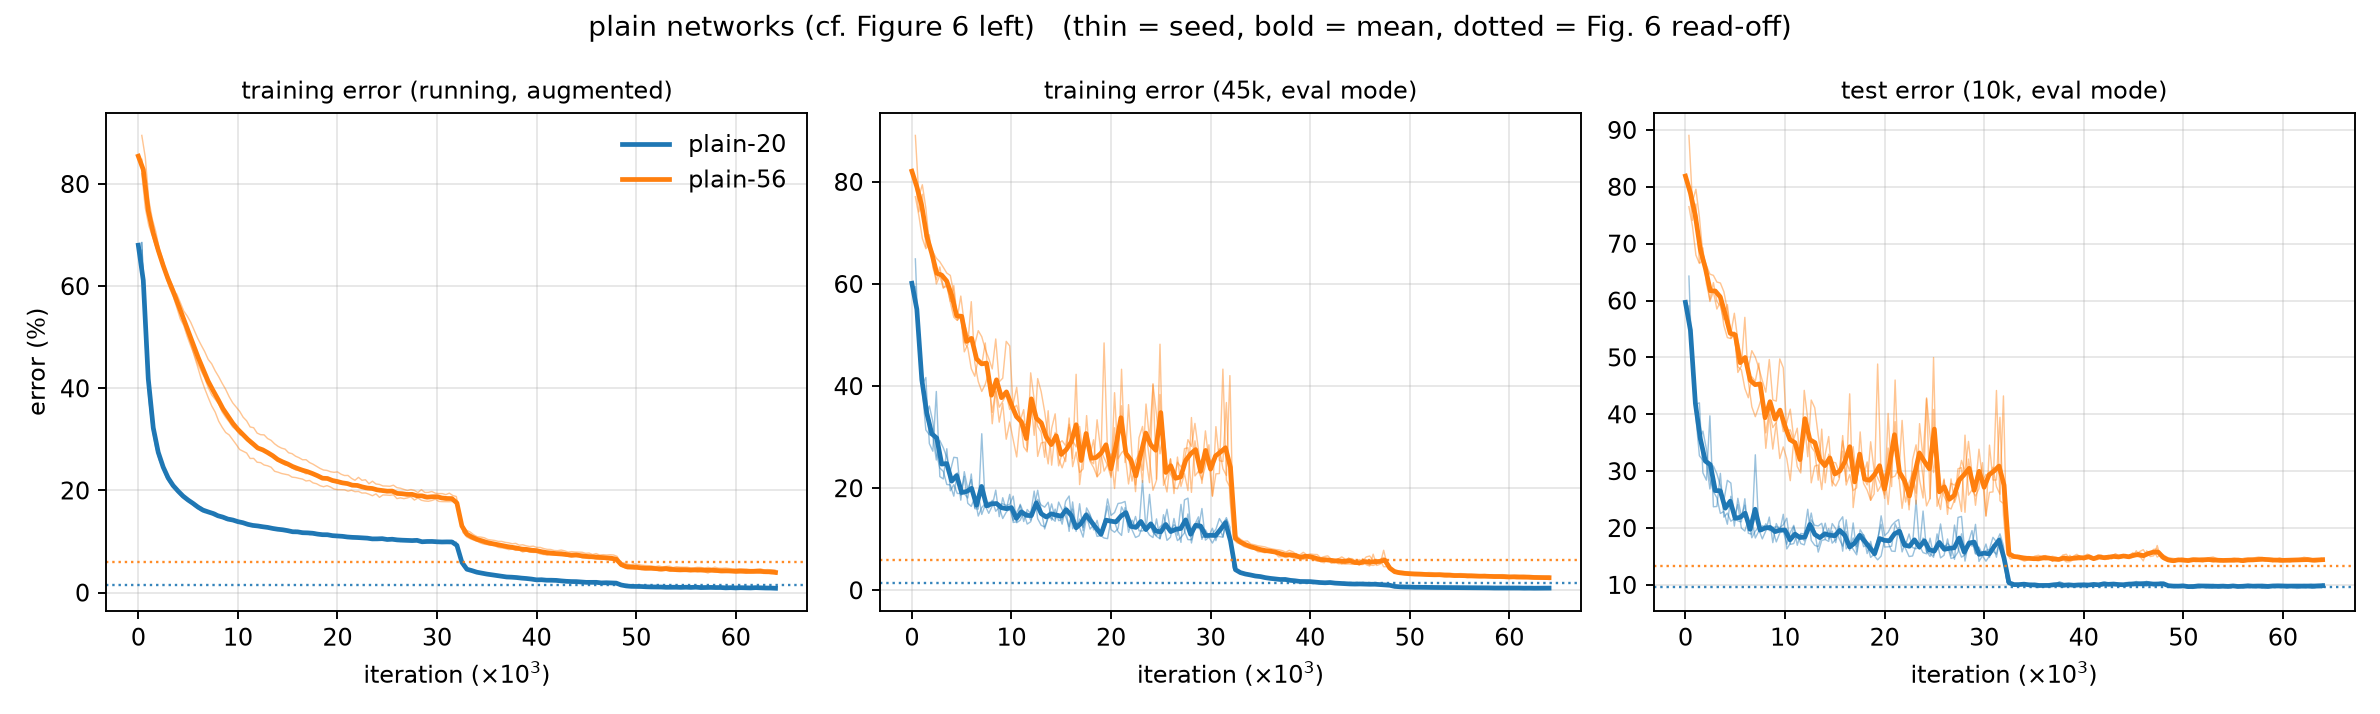
\includegraphics[width=\textwidth]{figures/fig6_plain.png}
\end{center}
\vspace{-8pt}
\begin{center}
\footnotesize{Plain networks. Thin lines are individual seeds, the bold line is
the mean over the three seeds. Dotted horizontal lines are the values we read
off Figure~6 of the paper: 1.5\% and 9.7\% for plain-20, 5.9\% and 13.3\% for
plain-56. The two drops are the learning-rate divisions at 32{,}000 and
48{,}000 iterations.}
\end{center}
\caption{Training and test error of the plain networks, against the paper's
Figure~6 (left).}\label{fig:plain}
\end{figure}

\begin{figure}[p]
\begin{center}
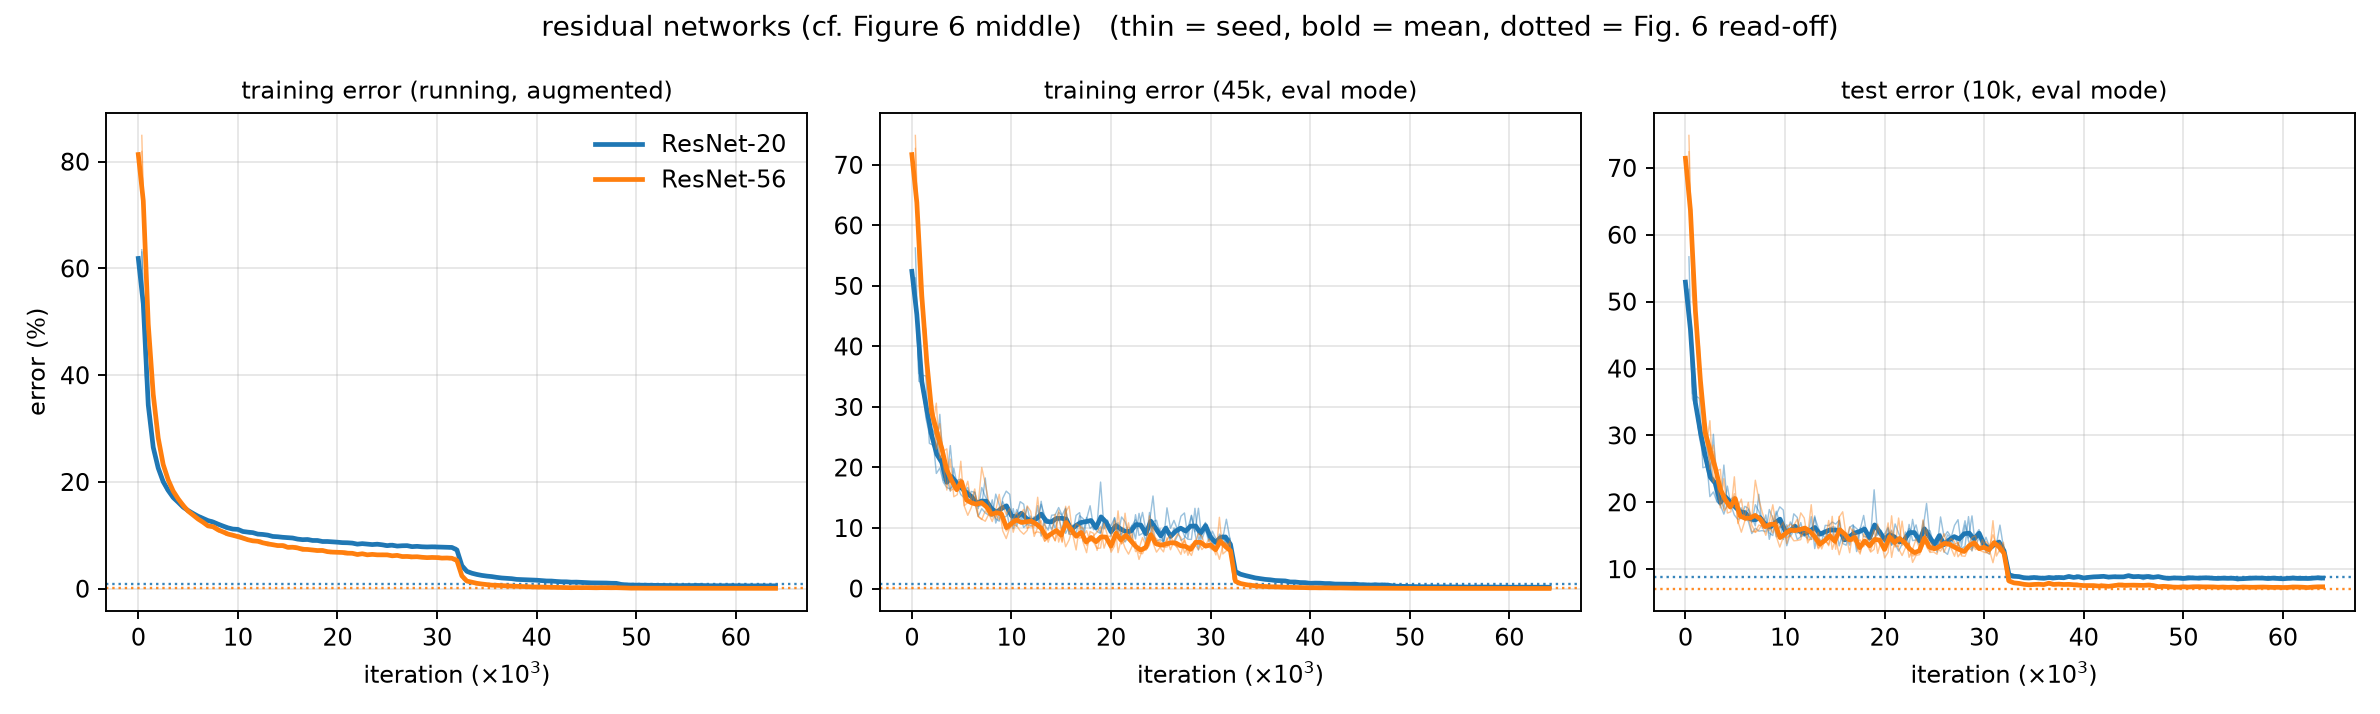
\includegraphics[width=\textwidth]{figures/fig6_resnet.png}
\end{center}
\vspace{-8pt}
\begin{center}
\footnotesize{Residual networks, same layout. Dotted lines are the read-offs
from Figure~6: 0.8\% and 8.8\% for ResNet-20, 0.1\% and 7.0\% for ResNet-56.}
\end{center}
\caption{Training and test error of the residual networks, against the paper's
Figure~6 (middle).}\label{fig:resnet}
\end{figure}

\section{Extension: does the degradation survive a tuned learning rate?}
\label{sec:extension}

\subsection{The question and the hypothesis}

The paper trains the 20- to 56-layer networks with one learning-rate schedule
and gives a warm-up only to the 110-layer network. If 56 layers simply need a
smaller step size than 20, the degradation could be a tuning artefact rather
than a property of depth. The extension asks whether the degradation remains
when each depth is allowed its own initial learning rate.

Our hypothesis, written before any of these runs were started: \emph{the
learning rate selected for plain-56 is lower than the one selected for
plain-20, and the degradation remains after tuning.} The second half matters
more than the first: a lower rate that still leaves the deep network worse
would show that depth costs something that a step size cannot buy back.

\subsection{The controlled experiment}

Only one thing is varied: the initial learning rate, over $\{0.01, 0.03, 0.1,
0.3, 0.5\}$. Everything else is held fixed, including the two divisions by ten
at 32{,}000 and 48{,}000 iterations, the full 64{,}000-iteration schedule
without warm-up, the 45k/5k split, and the augmentation. Both depths are tuned
in exactly the same way. Each grid point is one run with seed 0; the run at 0.1
is the replication's own seed 0, so the grid adds eight new runs.

Selected by a pre-registered rule: the lowest \emph{training} error in
evaluation mode at the last iteration. This deliberately departs from selecting
on the validation set, because the question is about optimisation, not
generalisation. Validation errors are reported in Table~\ref{tab:tuning} but are
not used for the choice.

\begin{table}[h]
\centering
\begin{tabular}{@{}lrrrrl@{}}
\toprule
Depth & Initial lr & Training 45k & Validation 5k & Test 10k & Status \\
\midrule
20 & 0.01 & 1.01 & 11.36 & 12.26 & --- \\
20 & 0.03 & 0.45 & 9.96 & 10.79 & --- \\
20 & \textbf{0.1} & \textbf{0.43} & 9.14 & 10.15 & selected \\
20 & 0.3 & 0.43 & 8.82 & 8.82 & tied \\
20 & 0.5 & 0.64 & 9.34 & 9.59 & --- \\
\midrule
56 & 0.01 & 3.91 & 15.92 & 16.94 & --- \\
56 & \textbf{0.03} & \textbf{1.94} & 15.10 & 15.61 & selected \\
56 & 0.1 & 2.81 & 13.96 & 14.58 & --- \\
56 & 0.3 & --- & --- & --- & \textbf{diverged, iter.\ 23} \\
56 & 0.5 & --- & --- & --- & \textbf{diverged, iter.\ 14} \\
\bottomrule
\end{tabular}
\caption{The tuning grid, one seed per setting. Errors in percent at
iteration 64{,}000. The 20-layer entries at 0.1 are the replication's seed 0.}
\label{tab:tuning}
\end{table}

\subsection{What the grid shows}

The selected rates are 0.1 for plain-20 and 0.03 for plain-56, so the first half
of the hypothesis holds: the deeper plain network wants a rate 3.3 times
smaller.

The stronger evidence is in the divergences. At 0.3 and 0.5 plain-56 does not
merely do badly, it stops training: the loss becomes NaN at iterations 23 and
14. Both were re-run on their own afterwards and diverged at exactly the same
iterations, so this is reproducible numerics and not an artefact of running
several jobs at once. plain-20 at the same two rates trains normally. The
practical statement is blunt: for this architecture and schedule, there is a
region of learning rates in which a 20-layer network trains and a 56-layer one
does not train at all, and it is a region the paper's single shared schedule
sits inside.

Figure~\ref{fig:tuning} shows the same thing visually, and also shows why the
selection rule needs to be read carefully.

\begin{figure}[p]
\begin{center}
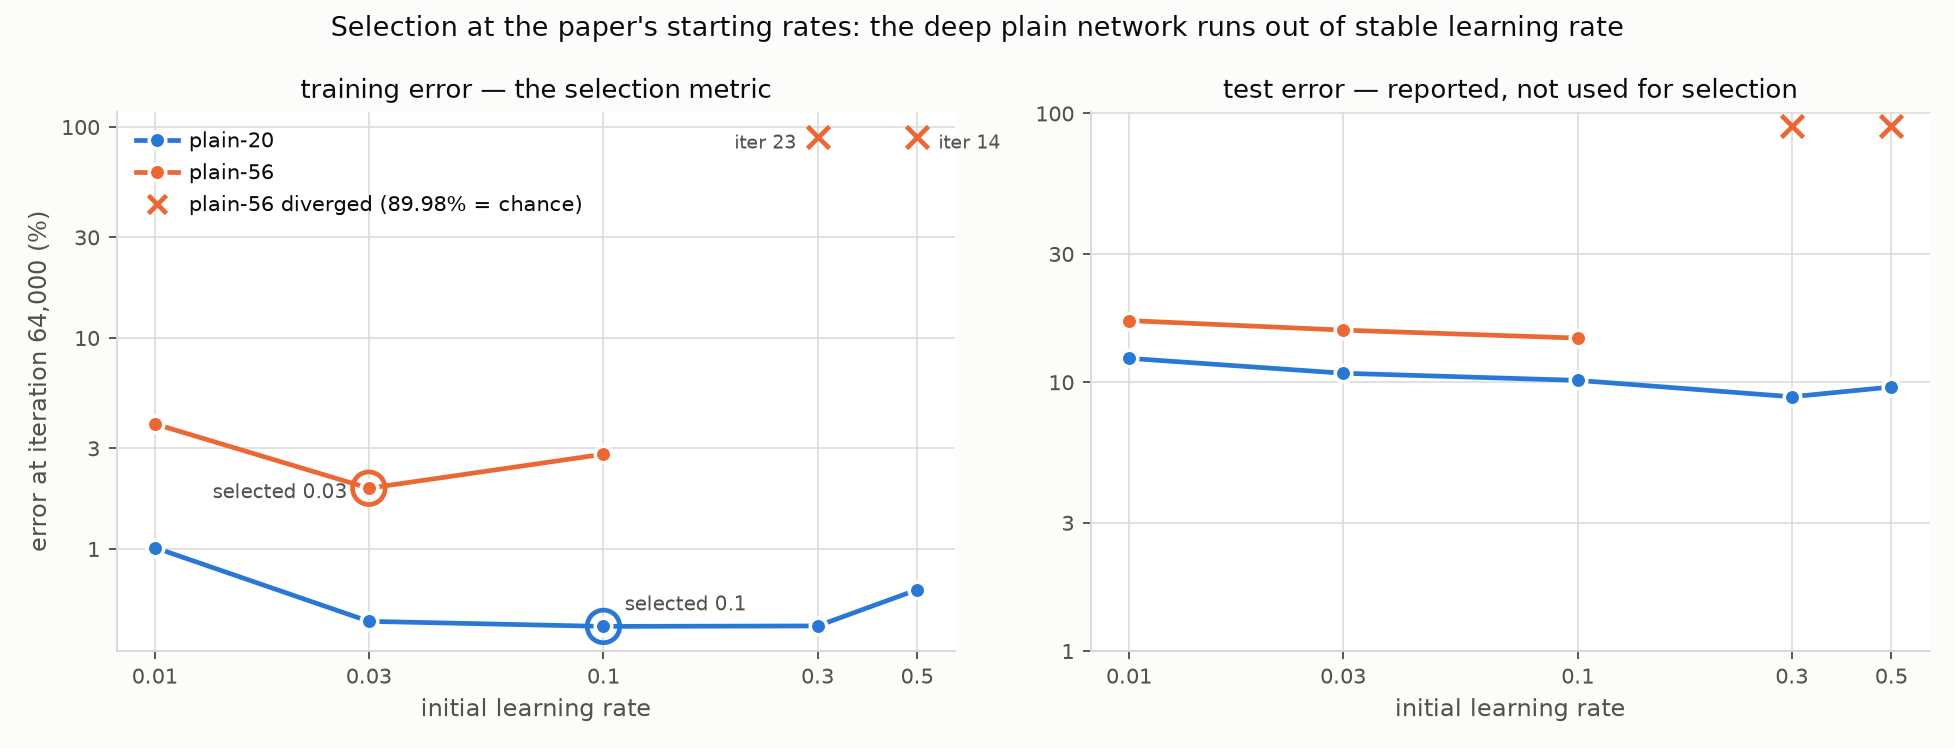
\includegraphics[width=\textwidth]{figures/extension_a_lr.png}
\end{center}
\vspace{-8pt}
\begin{center}
\footnotesize{Final error against the initial learning rate, log scale on both
axes. Crosses are the plain-56 runs that diverged, drawn at their recorded
error of 89.98\%, which is chance for ten classes. The ringed points are the
selections.}
\end{center}
\caption{The tuning grid. The left panel is the selection metric, the right
panel reports test error and is not used for the choice.}\label{fig:tuning}
\end{figure}

Two qualifications belong in the record rather than in a footnote. First, the
plain-20 selection is nominal: 0.1 and 0.3 differ by 0.002 \pp{} on the
selection metric, which is far below the 0.11-point seed spread of plain-20
itself, and the two should be described as tied. Second, a grid of one seed per
setting cannot support a claim about differences between grid points on test
error. Comparing 0.03 and 0.1 for plain-56 on the tuning runs alone makes 0.1
look better (14.58 against 15.61), while the three-seed sets in the next section
make the selected rate look slightly better (14.18 against 14.43). Neither
ordering is meaningful; only the selection, which is defined on a quantity that
is measured consistently, is being used.

\subsection{Three seeds at the selected rates}

The handout requires three seeds for any comparison a conclusion is drawn from,
and a tuning run does not count as one of them. plain-20 selects 0.1, which the
topic card allows to be the replication's own seeds, so those three runs serve
directly. plain-56 selects 0.03, so its tuning run is excluded and three fresh
seeds were trained.

\begin{table}[h]
\centering
\begin{tabular}{@{}lrrrr@{}}
\toprule
Network (selected lr) & Seed & Training 45k & Validation 5k & Test 10k \\
\midrule
plain-20 (0.1) & 0, 1, 2 & \textbf{0.43} & 9.20 & \textbf{9.87} \\
plain-20 (0.1) & spread & 0.11 & 0.38 & 0.60 \\
\midrule
plain-56 (0.03) & 1, 2, 3 & \textbf{1.70} & 13.53 & \textbf{14.18} \\
plain-56 (0.03) & spread & 0.52 & 2.06 & 2.44 \\
\bottomrule
\end{tabular}
\caption{Means and spreads over three non-tuning seeds at each network's
selected rate.}\label{tab:tuned}
\end{table}

The degradation remains. Training error: $1.70 - 0.43 = +1.27$ \pp{} against a
larger spread of 0.52, so real. Running training error: $3.05 - 0.85 = +2.20$
\pp{} against 0.92, so real. Test error: $14.18 - 9.87 = +4.31$ \pp{} against
2.44, so real.

The comparison the card asks for is with the replication at the shared rate of
0.1, where the training gap was 2.04 \pp. Tuning each depth separately reduces
the gap to 1.27 \pp{}, a little over a third smaller. The second half of the
hypothesis therefore holds too, and with a substantive reading: giving the deep
network its own learning rate recovers part of the loss, not all of it.

\section{Why: layer responses and gradients}

A result about optimisation should come with evidence about what is failing.
We measure two things on the trained seed-0 models, both on the 10{,}000 test
images.

Figure~\ref{fig:resp} repeats the measurement behind the paper's Figure~7: the
standard deviation of each layer's output, taken after batch normalisation. The
paper's reading is that plain networks have conspicuously smaller responses as
depth grows, while residual networks keep theirs comparable. Our models show
exactly that ordering: over the sorted curves, plain-56 sits systematically
below plain-20, and the residual curves are flatter than the plain ones.

\begin{figure}[p]
\begin{center}
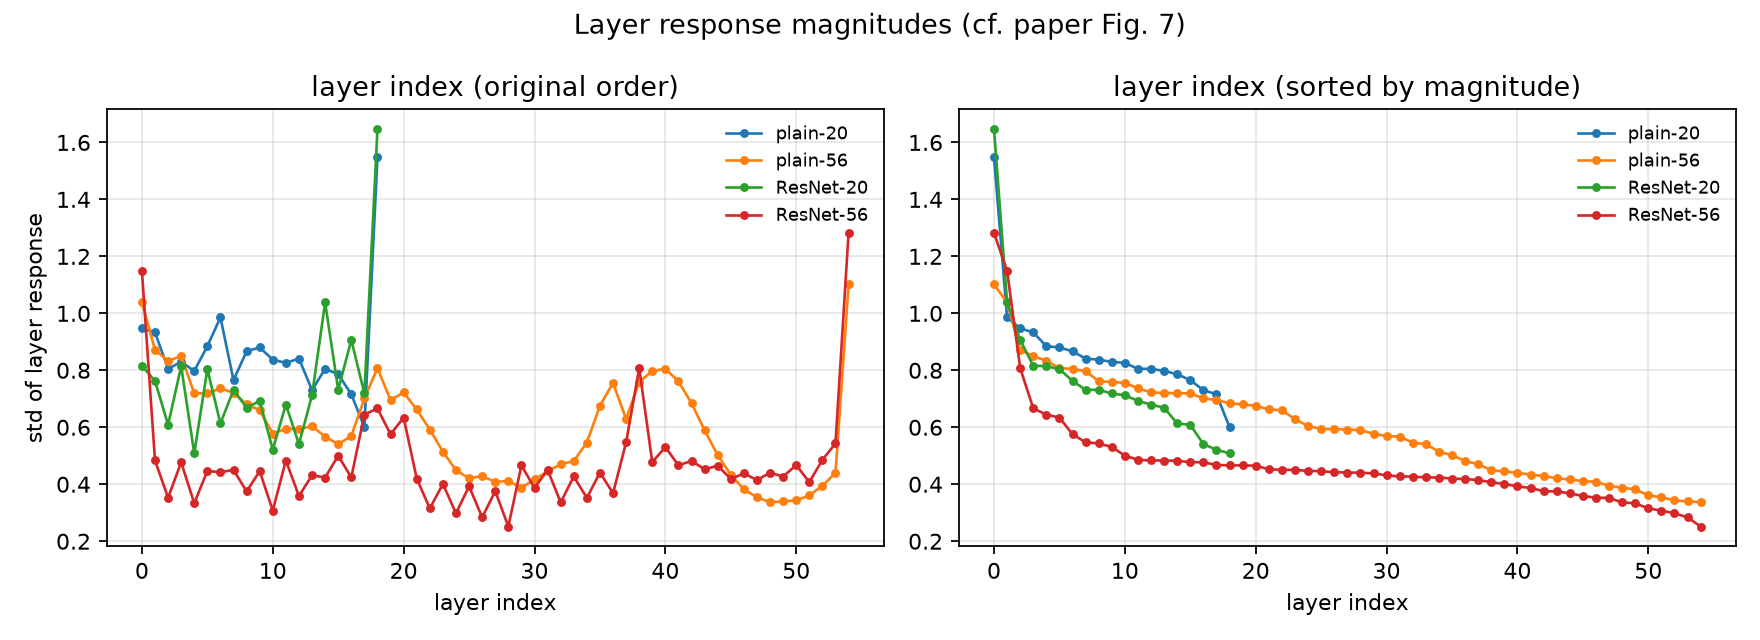
\includegraphics[width=\textwidth]{figures/fig7.png}
\end{center}
\vspace{-8pt}
\begin{center}
\footnotesize{Standard deviation of each layer's response, in layer order (left)
and sorted by magnitude (right), measured after batch normalisation on the test
set.}
\end{center}
\caption{Layer response magnitudes, after the paper's Figure~7.}\label{fig:resp}
\end{figure}

Figure~\ref{fig:grad} checks the paper's other argument, that gradients are not
vanishing. Taking one batch and one backward pass, the smallest per-layer
gradient norm is 0.12 for plain-56 against 0.24 for plain-20. The deeper plain
network's gradients are smaller, but they are not zero and they are not
exponentially suppressed: the degradation is not a vanishing-gradient story in
our models either.

\begin{figure}[p]
\begin{center}
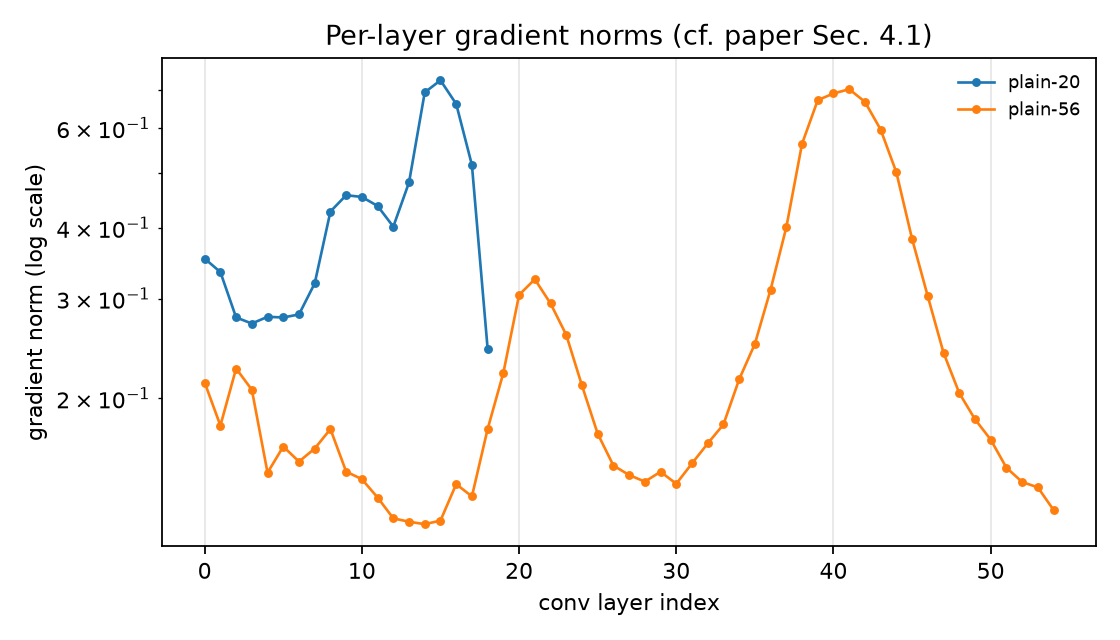
\includegraphics[width=0.78\textwidth]{figures/gradients.png}
\end{center}
\vspace{-8pt}
\begin{center}
\footnotesize{Per-layer gradient norm of the convolutional weights, log scale,
one batch, after the first backward pass.}
\end{center}
\caption{Per-layer gradient norms for the two plain networks.}\label{fig:grad}
\end{figure}

Two limits on these measurements must be stated. They are single-batch, single-
step diagnostics on one seed, not a study of training dynamics, and the
response measurement depends on the batch statistics used in evaluation mode.
They are consistent with the paper's account; they do not independently establish
its causal claim.

\section{Discussion}
\label{sec:discussion}

\textbf{The plain-56 gap.} Three of our four reproduced numbers are within
0.4 \pp{} of the published value; plain-56 is 1.13 \pp{} worse. It is not seed
noise: the seed spread at that depth is only 0.23 \pp{} on test error, so the
gap is systematic for our setup. The most likely single cause is the training
set. We train on 45{,}000 images; if the paper's networks saw all 50{,}000,
that explains a uniform penalty, and plain-56 is the network most sensitive to
it because it is the one that is furthest from fitting even the 45{,}000. The
argument is weakened by the fact that the other three networks are closer to
their published values than such a uniform penalty would predict, so we do not
claim it is the whole story. The honest summary is that we reproduce the
paper's \emph{ordering} precisely and its worst plain number only approximately.

\textbf{Tuning is not the explanation.} The natural objection to a degradation
result is that the deep network is simply mis-tuned. Our extension tests that
directly and finds it insufficient: even with its own selected rate, plain-56
is 1.27 \pp{} behind plain-20 on training error against a 0.52 spread. Tuning
buys back about a third of the gap. The divergence behaviour sharpens the point
--- the deep plain network cannot even use the rates the shallow one uses.

\textbf{Reproducibility is itself part of the result.} The seed spread at the
selected rates is 2.44 \pp{} on test for plain-56 and 0.60 for plain-20. The
deeper plain network is worse on average and much less stable run to run. A
single-run comparison at this depth, which is what the paper's Table~6 provides,
carries an uncertainty that the paper does not report.

\textbf{What the residual connections change.} Our residuals gain 1.31 \pp{}
over their plain counterparts at depth 56 in the same direction as the paper's
1.78, and remove the response shrinkage that Figure~\ref{fig:resp} shows. We
did not test the paper's options B and C for the shortcut, so we can say that
option A works, not that it is the best option.

\section{Conclusion}

\subsection*{What our experiments show}

\begin{itemize}
\item On CIFAR-10 with the paper's recipe, a plain 56-layer network has a higher
training error than a plain 20-layer one, by 2.04 \pp{} in evaluation mode and
3.10 \pp{} on augmented batches, both larger than the seed spread. The
degradation is reproduced, and it is an optimisation failure rather than
overfitting.
\item Adding identity shortcuts reverses the ordering: ResNet-56 is 1.31 \pp{}
better than ResNet-20 on test error against a 0.34 spread, in the same direction
as the paper's 1.78.
\item The degradation survives tuning the learning rate separately for each
depth. The selected rate is lower for the deeper network (0.03 against 0.1),
plain-56 diverges outright at 0.3 and 0.5 while plain-20 trains there, and after
tuning the training gap is still 1.27 \pp{} against a 0.52 spread.
\item Layer responses shrink with depth in the plain networks and stay flatter
in the residual ones, and gradients do not vanish in either plain network. Both
are consistent with the paper's account.
\end{itemize}

\subsection*{What our experiments do not show}

\begin{itemize}
\item \emph{Why} residual connections help. Our response and gradient
measurements are single-batch diagnostics consistent with the paper's account;
they do not identify a mechanism, and we did not test the paper's options B and C.
\item That the paper's recipe produces 13.3\% for plain-56. We get 14.43\%. The
most plausible cause is the 45{,}000-image training set, but we did not run the
50{,}000-image variant, so this remains a hypothesis.
\item Anything about rates between or beyond the five grid points, or about
differences in test error between grid points: the grid is one seed per setting
by design, and the run-to-run spread at depth 56 is larger than those
differences.
\item Anything about a schedule longer than 64{,}000 iterations, other datasets,
other widths, or other shortcut options. The extension varies one factor only.
\end{itemize}

\clearpage
\section*{AI use declaration}
We used Claude Code (Anthropic) as a coding and writing assistant. It wrote the
training, evaluation, plotting and summarisation code, and drafted this report
from the team's own experiment outputs. The recipe and protocol were taken from
the paper and the topic card by the team; every number in this report is
generated by our scripts from the runs' output files rather than typed by hand;
all code and experiments are run and understood by the team, and every member
can explain every line and every plot, as the course requires.

\section*{Contribution statement}

\begin{center}
\begin{tabular}{@{}llp{7.6cm}@{}}
\toprule
\textbf{Member} & \textbf{Student ID} & \textbf{Contribution} \\
\midrule
Chen Letian & 2330026013 & \emph{to be completed by the team} \\
Zhang Yiyang & 2430024331 & \emph{to be completed by the team} \\
Liu Chuanliang & 2330013021 & \emph{to be completed by the team} \\
Liu Yilin & 2430026139 & \emph{to be completed by the team} \\
\bottomrule
\end{tabular}
\end{center}

\section*{References}
\begin{enumerate}
\item K.~He, X.~Zhang, S.~Ren, J.~Sun. Deep residual learning for image
recognition. CVPR 2016.
\item A.~Krizhevsky. Learning multiple layers of features from tiny images.
Technical report, University of Toronto, 2009.
\item S.~J.~D.~Prince. \emph{Understanding Deep Learning}. MIT Press, 2023.
\S11.1--11.4.
\item D.~Balduzzi, M.~Frean, L.~Leary, J.~P.~Lewis, K.~W.-D.~Ma, B.~McWilliams.
The shattered gradients problem: if resnets are the answer, then what is the
question? ICML 2017.
\end{enumerate}

\noindent\footnotesize{Code, run outputs and the scripts that produce every table
and figure in this report are at \texttt{github.com/\allowbreak
v68md6ttb2-ux/\allowbreak COMP4163-ResNet-Degradation}.}

\end{document}
